\documentclass[12pt, a4paper]{article}

\usepackage{cmap} 
\usepackage[T2A]{fontenc} 
\usepackage[utf8]{inputenc} 
\usepackage[english,russian]{babel}
\usepackage{amsmath}
\usepackage{graphicx}
\graphicspath{ {./images/} }
\title{Дендрограмма}
\date{}

\begin{document}
\maketitle
\hspace{0.5cm} Дендрограмма – визуализатор, используемый для иерархической кластеризации. Дендограмма наглядно показывает связь между отдельными объектами и кластерами. Количество уровней дендрограммы зависит от количества шагов в алгоритме. 
С помощью методов машинного обучения и секвенирования ДНК, ученым удалось выяснить, принадлежат большие панды к енотовым или медвежьим. 
С помощью иерархической кластеризации можно построить филогенетическое дерево животных, которое, в свою очередь, показывает, что большие панды ближе к медведям, чем к енотам 

\begin{figure}[!htb]
\begin{center}
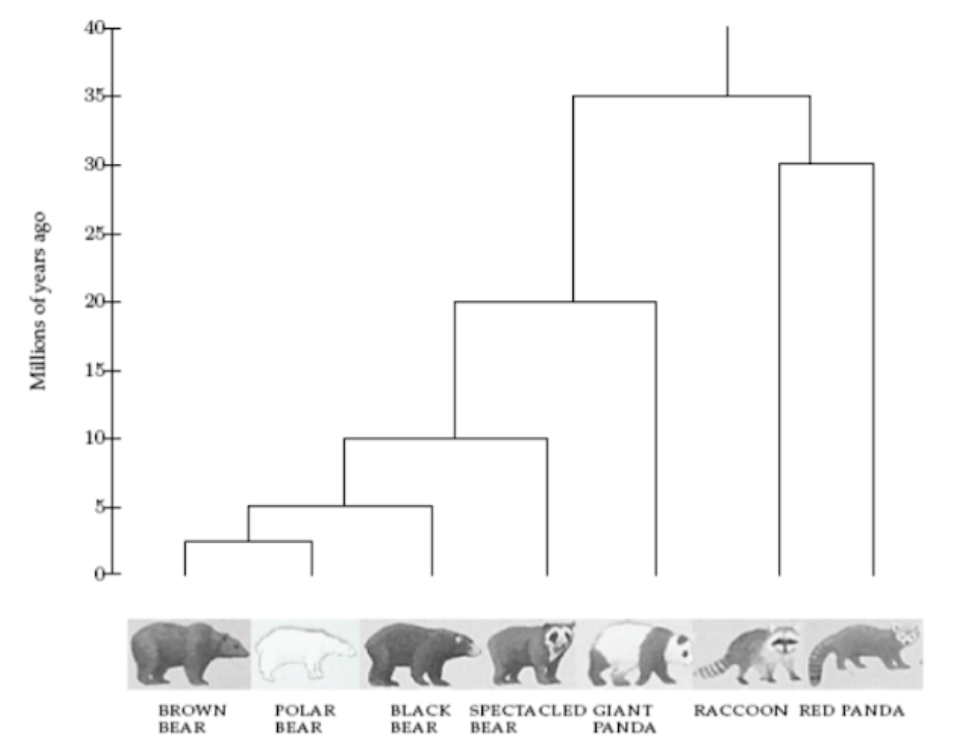
\includegraphics[width=110mm]{e.png}
\end{center}
\caption{}
\end{figure}



\end{document}